\scanpage{212}
\[
\varphi_1(X_0^{(i)})=\text{\textcircled{$\xi_i,\ i\geq1$}}\qquad\boxed{\xi_i\xi_j=c_{ij}\xi_{i+j}}\quad(i,j\geq1)
\]
\[
\varphi_1(dX_0)=d\xi_1\qquad\boxed{d\xi_i=\xi_{i-1}d\xi_1}\qquad\boxed{\xi_i\in\unsure{S'}\{X_0\}^+}
\]
\[
\xi_i=A_i+B_i\,dX_0\qquad A_i,B_i\in S'\{X_0\}\qquad A_i\in S'\{X_0\}^+
\]
\[
dA_i=A_{i-1}A'_1
\]
\[
A_i=\xi_1^{(i)}
\]
\figure{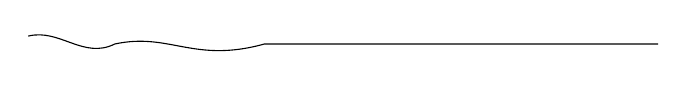
\begin{tikzpicture}\draw (0,0.1) .. controls (0.4,0.2) and (0.7,-0.2) .. (1.1,0) .. controls (1.8,0.15) and (2.1,-0.25) .. (3,0) -- (8,0);\end{tikzpicture}}
\uline{Remarque} On voit donc que tt $\varphi_1$ se met de façon \uline{unique} sous la forme $\psi_1\circ\overline\varphi_0$, où $\overline\varphi_0$ est l'hom qui prolonge $\varphi_0$ ($\overline\varphi_0(X_0^{(i)})=X_0^{(i)}$, $\overline\varphi_0(dX_0)=\deleted{\unsure{\varphi}}dX_0$) et $\psi_1$ est un $S'$-endom de la $S'$-alg. diff. $A_{S'}$, compatible avec l'augmentation.

Il faut maintenant exprimer la compatibilité de $\varphi_1$ aux augmentations $\beta$ \inserted{(si $S=k\{T\},S'=k'\{T\}$)} ($X_0\longmapsto T$, \inserted{et $X_0^{(i)}\longmapsto T^{(i)}$} $dX_0\longmapsto0$).
On trouve que l'on doit avoir
\[
\beta_{S'}(\xi_i)=\varphi_0(T^{(i)})\quad\text{i.e.}\quad\deleted{\unsure{A_{S'}}}\beta_{S'}(A_i)=\overline\varphi_0(T^{(i)})
\]
ce qui revient, puisque $A_i=A_1^{(i)}$, à
\inserted{\[
\left\{\begin{array}{l}
\beta_{S'}(A_1)=\overline\varphi_0(T)\\
\varphi_0(T^{(i)})=\varphi_0(T)^{(i)}
\end{array}\right.
\]}
donc on a
\[
A_1\deleted{\unsure{\{X_0\}}}=X_0+f\deleted{\unsure{\{X_0\}}}
\]
où $f\in\mathcal A_{\deleted{\unsure{*}}1}\simeq k\{X_0,X_1\}$ est donné par
\[
f=\sum_{i\geq1,j\geq1}X_0^{(i)}X_1^{(j)}
\]
La \uline{remarque} ci-dessus se prolonge \unsure{en}
\margin{211}
